\documentclass{beamer}
\mode<presentation> {\usetheme{Frankfurt}}

\usepackage{graphicx} % Allows including images
\usepackage{amsmath,amsthm,amsfonts,graphicx,bm,bbm,wrapfig}
\usepackage{amssymb}
\usepackage{enumerate}
\usepackage{mathrsfs}
\usepackage{graphicx}
\usepackage{color}
\usepackage{breqn}
\usepackage{subfigure}
\usepackage{float}
\usepackage{color}

\title[HPC Final Project]{HPC final project: \\
	Ewald summation on stokes potential} % The short title appears at the bottom of every slide, the full title is only on the title page

\author{Zhe Chen, Guanchun Li} % Your name
\institute[CIMS] % Your institution as it will appear on the bottom of every slide, may be shorthand to save space
{
Courant Insititute of Mathematical sciences \\ % Your institution for the title page
\medskip
\textit{zc1291@nyu.edu, gl1705@nyu.edu} % Your email address
}
\date{\today} % Date, can be changed to a custom date

\begin{document}

\begin{frame}
\titlepage
\end{frame}

\section{Background of Ewald Summation}
\begin{frame}{Periodic Stokes potentials}
Consider a system of $N$ point sources at location $\mathbf{x}_n$ with strength $\mathbf{f}_n$, in the periodic setting, the velocity field is 
\begin{equation}
\mathbf{u}(\mathbf{x}) = \sum_{n=1}^{N} \sum_{\mathbf{p}} \mathbf{S}(\mathbf{x - x_n + p}) \mathbf{f}_n, \label{eq:stokes_velocity_field}
\end{equation} 
with $\mathbf{S}$ the Oseen-Burgers tensor:
\begin{equation}
\mathbf{S}(\mathbf{x}) = \frac{\mathbf{1}}{|\mathbf{x}|} + \frac{\mathbf{x x}}{|\mathbf{x}|^3}.
\end{equation}
 
where $\mathbf{p}$ form the discrete set $\{[iL_x \ jL_y \  kL_z]:(i, j, k) \in \mathbb{Z}^3\}$.\\

\textbf{Warning: Eq.\eqref{eq:stokes_velocity_field} decays as $1 / |\mathbf{x}|$!} \\

We need \textbf{Ewald summation} to compute this.
\end{frame}

\begin{frame}{Ewald summation}
\begin{eqnarray}
\mathbf{u}(\mathbf{x}_m) = &  \sum_{n=1}^{N} \sum_{\mathbf{p}} \mathbf{A}(\xi, \mathbf{x_m - x_n + p}) \mathbf{f}_n  - \mathbf{u}_{\text{self}} \label{eq:ewald_sum} \notag \\ 
+ &  \frac{1}{V} \sum_{\mathbf{k} \neq 0} \mathbf{B}(\xi, \mathbf{k}) e^{-k^2/4\xi^2}\sum_{n=1}^{N} \mathbf{f}_n e ^{-i \mathbf{k} \cdot (\mathbf{x}_m - \mathbf{x}_n)} 
\end{eqnarray} 

By the formulation by Hasimoto \cite{Hasimoto1959}, we have
\begin{eqnarray}
& \mathbf{A}(\xi, \mathbf{x}) = 2 \left(\frac{\xi e^{-\xi^2 r^2}}{\sqrt{\pi} r^2} + \frac{\text{erfc}(\xi r)}{2 r^3}\right) (r^2 \mathbf{I} + \mathbf{x x}) - \frac{4 \xi}{\sqrt{\pi}} e^{-\xi^2 r^2} \mathbf{I} \\
& B(\xi, \mathbf{k}) = 8 \pi \left(1 + \frac{k^2}{4 \xi^2}\right) \frac{1}{k^4}(k^2 \mathbf{I} - \mathbf{k k})\\
& \mathbf{u}_{\text{self}}(\mathbf{x}_m) = \frac{4 \xi}{\sqrt{\pi}} \mathbf{f}_m
\end{eqnarray}
$\xi$ is a positive constant known as the \textbf{Ewald parameter}.
\end{frame}

\section{Description of Algorithms}

\begin{frame}{Acceleration \& parallelization}
\begin{itemize}
	\item Compute $u^F$ (k-space) by FFT \\
	\begin{equation}
	\mathbf{u}^F (\mathbf{x}_m) = \frac{1}{V} \sum_{\mathbf{k} \neq 0} \mathbf{B}(\xi, \mathbf{k}) e^{-k^2/4\xi^2} \left(\sum_{n=1}^{N} \mathbf{f}_n e ^{i \mathbf{k} \cdot \mathbf{x}_n} \right)e ^{-i \mathbf{k} \cdot \mathbf{x}_m}
	\end{equation}
	is the combination of two steps of NuFFT (Non-uniform FFT).
	
	\textbf{Can be done efficiently by Gaussian Gridding \& FFT!}
	\begin{itemize}
		\item \textbf{Gaussian Gridding}: \\
		Compute $ \sum_{n=1}^N \mathbf{f}_n e^{-2 \xi^2 |\mathbf{x} - \mathbf{x}_n|_{\ast}^2 / \eta}$ \\
		Can be accelerated with Greengard's trick \cite{Greengard2004} and  OpenMP!
		\item \textbf{FFT}: \\
		Can be done efficiently by CuFFT (GPU) / FFTW (CPU) !
	\end{itemize}

	\item Accelerate $u^R$ (real space) by OpenMP 
\end{itemize}

\end{frame}

\begin{frame}{Important Parameters \& Error bound}
Free parameters:
\begin{itemize}
	\item $\xi$ : Ewald parameter
	\item $M$: Number of layers of k-space
	\item $p_{\infty}$: Number of layers of real-space
	\item $P, m$: control the error of truncated Gaussian function
\end{itemize}
Error Bound: \textbf{Spectral accurate!}
\begin{align}
E & = E^F + E^Q + E^R \\
E^F & \le C_F e^{-\frac{M^2 \pi^2}{4 L \xi^2}} \quad  \text{(truncation of k-space)}\\
E^Q & \le  4 e^{- \frac{\pi^2 P^2}{2 m^2 L^2}} + \text{erfc} (m / \sqrt{2}) \quad  \text{(quadrature)}\\
E^R & \le C_R (\frac{1}{\xi^2} + \frac{p_{\infty}}{\xi}) e^{-p_{\infty}^2 \xi^2}. \quad \text{(truncation of real space)}
\end{align}
\textbf{Ewald parameter $\xi$ trades off between real space and k-space!}
\end{frame}

\section{Implementation \& results}

\begin{frame}{Spectral convergence}
The three type of error versus the corresponding parameter, \\
all has \textbf{spectral convergence}!
\begin{figure}[H]\centering
	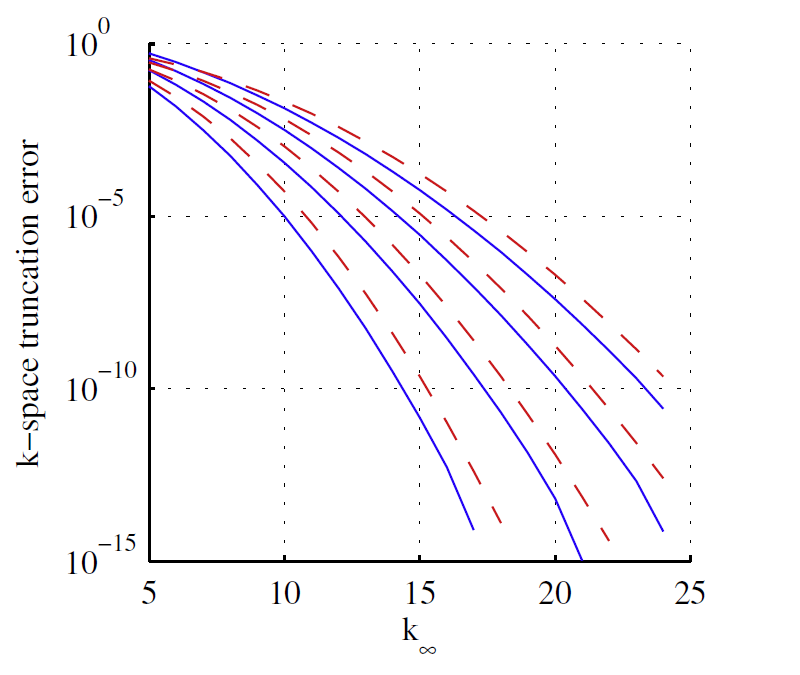
\includegraphics[width=.36\textwidth]{freq_error_vs_k}
	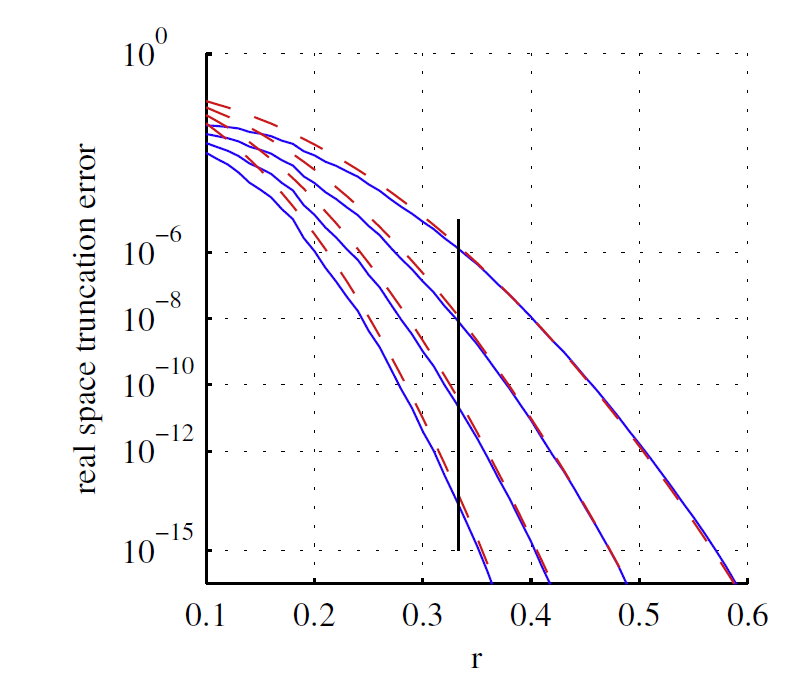
\includegraphics[width=.36\textwidth]{real_error_vs_r}
	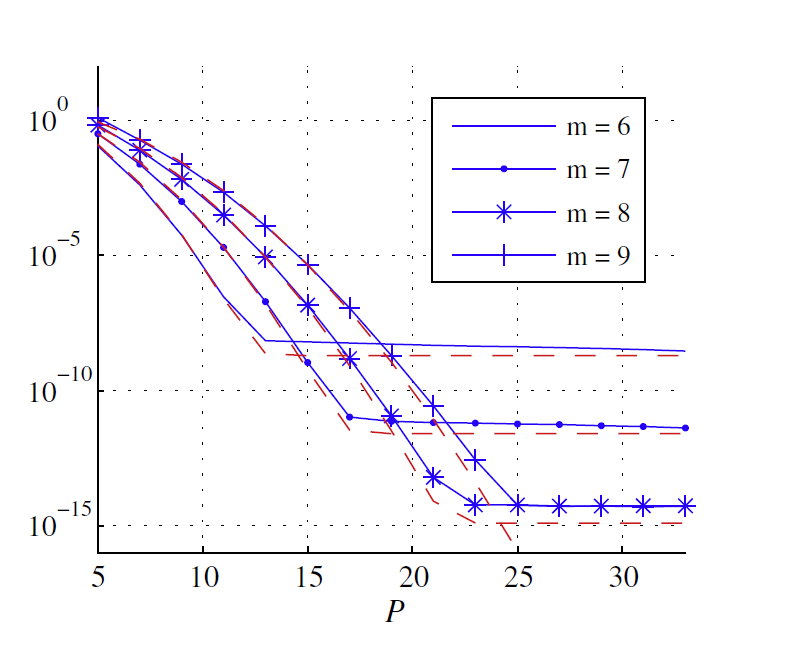
\includegraphics[width=.36\textwidth]{qudrature_error_vs_P}
\end{figure}
\end{frame}
\begin{frame}{Time Complexity \& Work load balance}
The total computational cost of the method is
\begin{equation}
\underbrace{O(NP^3)}_{\text{Gaussian gridding}} + \underbrace{O(M^3 \log(M^3))}_{\text{FFT + iFFT}} + \underbrace{O(M^3)}_{\text{Scaling on k-space}} + \underbrace{O(N^2 p_{\infty}^3)}_{\text{Real space}} + \underbrace{O(N)}_{self}
\end{equation}
if no FFT acceleration, the cost is
\begin{equation}
\underbrace{O(N^2M^3)}_{k-space} + \underbrace{O(N^2 p_{\infty}^3)}_{\text{Real space}} + \underbrace{O(N)}_{self}
\end{equation}
\textbf{Ewald parameter $\xi$ trades off between real space and k-space!}
\begin{itemize}
	\item Larger $\xi \rightarrow$ larger $M$, smaller $p_{\infty}$.
	\item Smaller $\xi \rightarrow$ smaller $M$, larger $p_{\infty}$.
\end{itemize}
How we choose the parameters:
\begin{itemize}
	\item \textbf{Balance the error} \\
	\item \textbf{Balance the time}
\end{itemize}
\end{frame}

\begin{frame}{Time Complexity result \& Scaling result}
\begin{figure}[H]\centering
	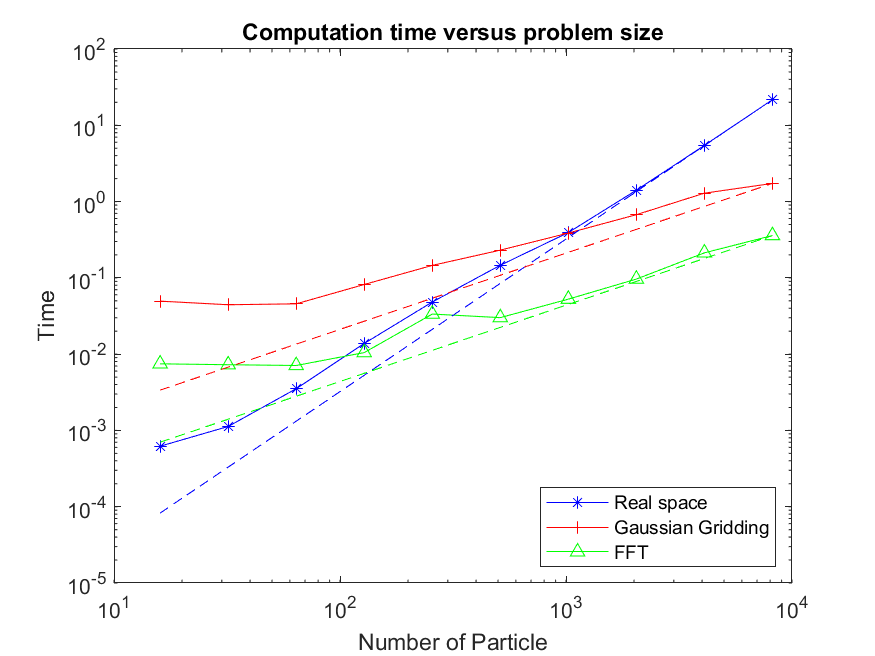
\includegraphics[width=.4\textwidth]{time_versus_np}
	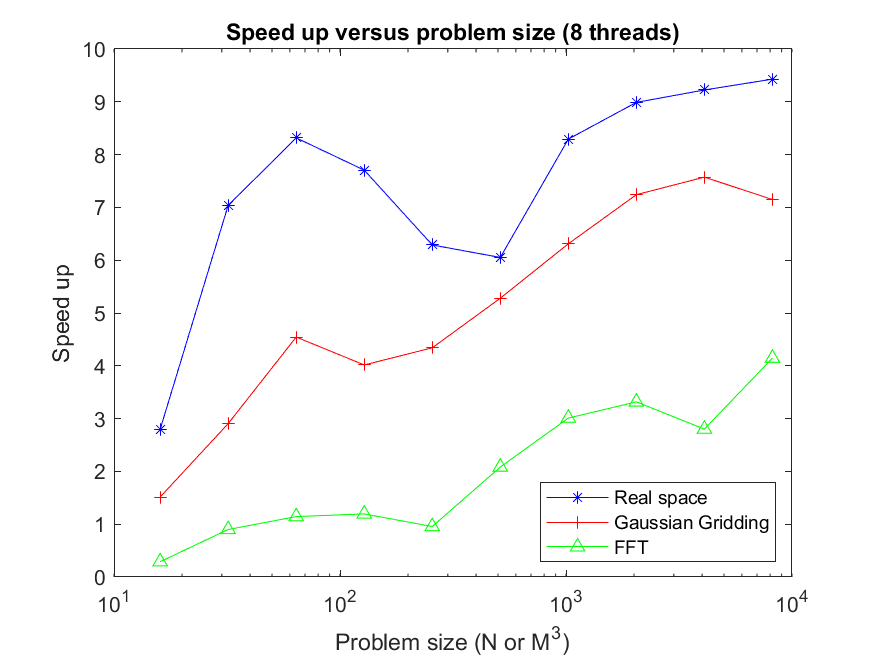
\includegraphics[width=.4\textwidth]{speed_up_versus_np}
\end{figure}
\end{frame}
\section{Acknowledgments}

\begin{frame}{References}
	\begin{thebibliography}{0}
		\bibitem{Greengard2004}
		Greengard, Leslie, and June-Yub Lee. "Accelerating the nonuniform fast Fourier transform." SIAM review 46.3 (2004): 443-454.
		\bibitem{Hasimoto1959}
		Hasimoto, Hidenori. "On the periodic fundamental solutions of the Stokes equations and their application to viscous flow past a cubic array of spheres." Journal of Fluid Mechanics 5.2 (1959): 317-328.
	\end{thebibliography}
\end{frame}

\end{document}